
% Sample file for AES paper
\documentclass{aes2e}

\usepackage{amsmath}
\usepackage{fourier}
\usepackage{graphicx}
\DeclareMathAlphabet{\mathcal}{OMS}{cmsy}{m}{n}
\SetMathAlphabet{\mathcal}{bold}{OMS}{cmsy}{b}{n}

% Metadata Information
\jyear{2010}
\jmonth{October}
\jvol{1}
\jnum{1}


\begin{document}

% Page heads
\markboth{A1LASTNAM AND A2LASTNAME}{SPECTRAL DELAY FILTERS}


% Title portion
\title{Parallel Triangle Counting Algorithms\thanks{To whom correspondence should be addressed Tel: +1-240-381-2383; Fax: +1-202-508-3799; e-mail: info@schtm.org}}

%Author Info.
\authorgroup{
\author{Michele Carloni}
AND \author{Riccardo Revalor}
\email{(carlonimichele3008@gmail.com)\quad\quad\quad\quad\quad\quad\quad\quad\quad\quad\quad\quad (s339423@studenti.polito.it)}
\affil{Politecnico di Torino, Computer Engineering}
}

%Abstract
\abstract{%
ABSTRACT: TODO}


\maketitle

%Head 1
\section{Mathematical definition of the problem}
Suppose that we have at our disposal a given graph $G = (V, E)$, where $G$ is the graph itself, $V$ denotes the set of all vertices (also called nodes), and $E$ represents the set of edges (also called links or arcs). An edge connects two nodes between them. The primary goal is to detect and count the number of triangles that can be formed inside the graph. More specifically, a \textbf{triangle} in graph $G = (V, E)$ is a set of three distinct vertices $\{u, v, w\} \subseteq V$ such that the edges $(u,v)$, $(v,w)$, and $(w,u)$ all exist in the set of edges $E$. This problem can be solved essentially using two distinct main approaches:
\subsection{Graph Traversal/Iterative Methods}
This category encompasses algorithms like the \textbf{Node Iterator} or the \textbf{Edge Iterator} that directly explore the graph, and at each iteration they try to look for the specific pattern that defines a triangle (three mutually connected vertices, as said before). They operate by iterating through parts of the graph (by scanning the list of either its nodes or edges) and checking for connections.
\subsection{Linear Algebra/Matrix Methods}
In this category, we mainly recall the \textbf{Matrix Multiplication} approach, which only works if the graph is represented by an adjacency matrix, which leverages matrix operations, specifically cubing (i.e. matrix multiplication) and trace computation, to get the exact number of triangles which can be created. Given the graph adjacency matrix $A$, this number is computed as $$\frac{1}{6} \text{ Trace}(A^3)$$ In graph terms, this trace represents the total count of all closed walks of length 3 in the graph, summed across all possible starting/ending vertices. 

\section{Node Iterator Algorithm, Forward Algorithm}
The simplest and most naive version of the Node Iterator Algorithm iterates over all nodes in the graph and, for each pair of neighbors of each node, checks whether they are connected by an edge. For each vertex, its \textbf{degree} $d(v)$ denotes its neighbors. If we have $V$ vertices, for each of them, we test unique pairs of neighbors that can be formed from $d(v)$ items. So, the overall complexity can be expressed as
\begin{align*}
\text{Complexity} &= \sum_{v \in V} \binom{d(v)}{2} \\
&= \sum_{v \in V} \frac{d(v)!}{2!(d(v)-2)!} \\
&= \sum_{v \in V} \frac{d(v) \cdot (d(v)-1) \cdot (d(v)-2)!}{2 \cdot 1 \cdot (d(v)-2)!} \\
&= \sum_{v \in V} \frac{d(v) \cdot (d(v)-1)}{2}
\end{align*}
In this project, we resorted to the so called \textbf{Forward Algorithm}, a variant which aims at improving complexity by iterating over vertices in a specific order, and efficiently queries their neighbors to identify potential triangle closures. We first implemented the \textbf{sequential} version of the algorithm, using \textbf{C++}, in which we can identify three main data structures used:
\begin{itemize}
    \item \textbf{Graph Representation:} How the graph's vertices and edges are stored, enabling efficient retrieval of a node's neighbors. We used and analyzed two primary representations: \textbf{adjacency matrices} (implemented as \texttt{std::vector<std::vector<int>>}) and \textbf{adjacency lists} (implemented as \texttt{std::map<int, std::vector<int>>} to handle potentially sparse or non-contiguous node IDs).
    \item \textbf{Auxiliary Sets (\textit{A[t]}):} Data structures used to store a specific subset of neighbors for each node (implemented as \texttt{std::vector<std::set<int>>}, where the outer vector is indexed by the node ID). These sets are then intersected (as defined in set theory) to identify the third vertex of a triangle.
    \item \textbf{Ordering/Ranks:} Structures (a sorted list of vertices and a map for ranks) to maintain and query the chosen ordering of vertices. Our implementation orders vertices by their degree (from highest to lowest) to optimize performance.
\end{itemize}
In the file \texttt{seq\_node\_it\_v1.cpp} there's the implementation using the adjacency matrix. An entry \texttt{adjacencyMatrix[i][j]} is 1 if there is an edge between vertex \texttt{i} and vertex \texttt{j}, and 0 otherwise. So, with N nodes, the space complexity to store the matrix is $\mathcal{O}\left(N^2\right)$. Neighbor retrieval is linear, as it's mandatory to scan the full row of the node inside the matrix. The auxiliary set is defined as \texttt{std::vector<std::set<int>> A}. When processing an edge \texttt{(s, t)}, the algorithm needs to find common elements between \texttt{A[s]} and \texttt{A[t]}. As \texttt{std::set} stores elements in sorted order, \texttt{std::set\_intersection} can be efficiently applied, resulting in a complexity of $\mathcal{O}\left(K_0 + K_1\right)$, being $K_0$ and $K_1$ the sets sizes. For the orderings we use \texttt{std::map<int, int> ranks} and \texttt{std::vector<int> orderedList}.Checking rank condition takes $\mathcal{O}\left(\log N\right)$ for map lookups, and we iterate through the whole \texttt{orderedList} so it takes $\mathcal{O}\left( N\right)$. \\
In the file \texttt{seq\_node\_it\_v2.cpp} we used the adjacency list, coded as a \texttt{std::map<int, std::vector<int>>} to better handle potentially sparse or non-contiguous node IDs. This version is \textbf{more efficient}: to find the neighbors of a vertex u, the algorithm performs a lookup in the map ($\mathcal{O}\left(\log N\right)$) and then copies the associated vector of neighbors ($\mathcal{O}\left( d(u)\right)$). This is significantly more efficient for sparse graphs than iterating an entire row of an adjacency matrix. \\
So, to resume the comparison between the two algorithms:
\begin{table}[htbp]
    \centering
    \caption{Summary of Sequential Forward Algorithm Implementation Complexities}
    \label{tab:forward_complexity_summary}
    \begin{tabular}{|l|l|}
        \hline
        \textbf{Graph Representation} & \textbf{Overall Time Complexity} \\
        \hline
        Adjacency Matrix & $\mathcal{O}(N^3 \log N)$ \\
        Adjacency List & $\mathcal{O}(M \cdot d_{max})$ \\
        \hline
    \end{tabular}
    \vspace{0.5em} % Adds a little space below the table
    \small
    Where $N$ is the number of vertices, $M$ is the number of edges, and $d_{max}$ is the maximum degree in the graph.
\end{table}

\section{Parallel Forward Algorithm}
In order to achieve better performances, we created two concurrent versions of the Forward Algorithm which iterates through graph nodes. As we did with the sequential version, the first one uses the adjacency matrix to represent the graph, whereas the latter employs the adjacency list. In the first, more naive and simple case, the part that gets parallelized is the Forward algorithm function. More in detail, the outer loop that iterates through the nodes in the ordered list is still sequential, running $N$ times, but the \textbf{iteration over each node neighbors t is parallelized}: this is achieved by dividing the neighbors of s into chunks, with each chunk processed by a separate worker thread using \texttt{std::async}. Each worker thread is responsible for computing intersections and updating the auxiliary sets (\texttt{A[t]}) for its assigned subset of neighbors. To protect data races and guarantee mutual exclusion over the variable to count the number of triangles and the auxiliary sets, we resorted to \textbf{mutexes} (efficiently used with C++ \textbf{RAII lock templates}). However, this first version does not improve the execution time of the algorithm compared to the sequential version, and the asymptotic worst-case complexity is unlikely to improve substantially. The mutexes \textit{de-facto} serialize operations on shared data, meaning that even with P threads, the core set operations effectively run in a serialized fashion due to \textbf{contention}. Moreover, the additional overhead related to thread creation (which becomes higher and higher as the number of threads used increases) actually \textbf{slows down} the process even more. During our tests, we observed that the excessive overhead was harmful to the performances of the algorithm:
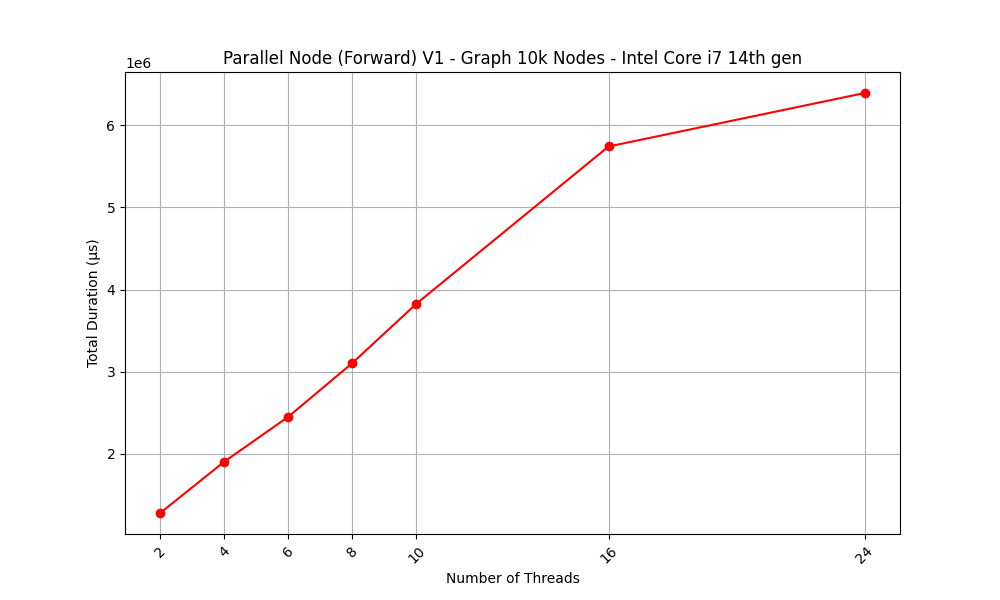
\includegraphics[width=0.52\textwidth, height=10cm, keepaspectratio]{charts/Parallel Node (Forward) V1 - Graph 10k Nodes - Intel Core i7 14th gen.png}
If we lower the number of vertices in the graph to, let's say, just 100, we can see that the parallel version of the algorithm becomes very inefficient, even counterproductive. This is because the time spent creating threads and managing context switching is presumably much higher than the computational gain achieved through parallel execution for such a small problem size. As a result, the overhead negates any potential speedup, making the sequential version the more performant choice:
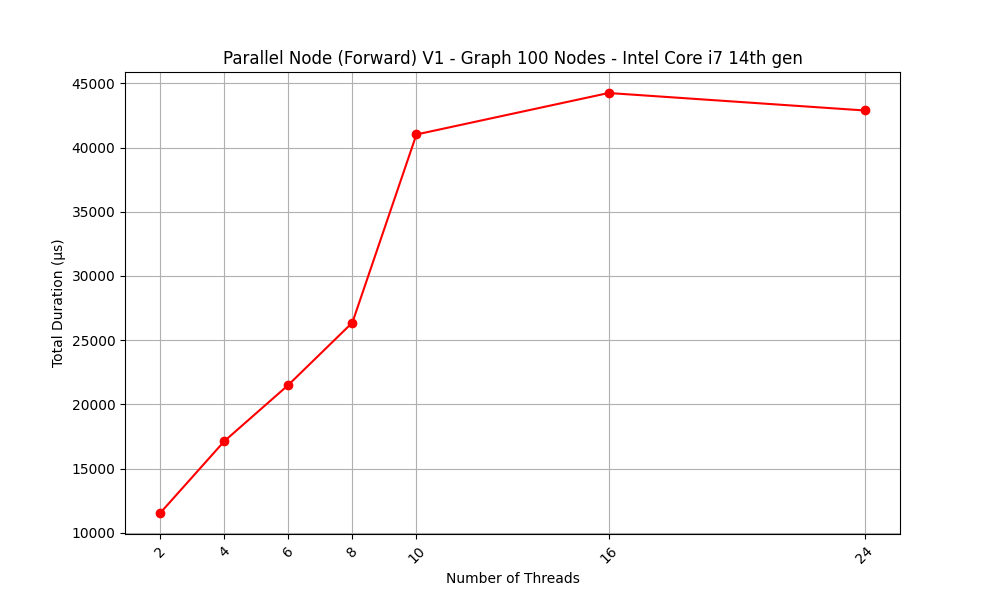
\includegraphics[width=0.52\textwidth, height=10cm, keepaspectratio]{charts/Parallel Node (Forward) V1 - Graph 100 Nodes - Intel Core i7 14th gen.png}

We can now show a much better and efficient version of the Parallel Forward Algorithm. Indeed, this second parallel version achieves \textbf{true parallel speedup of the parallelizable portion of the algorithm}, which is the $\mathcal{O}\left(M \cdot d_{max}\right)$) part. This approach uses an adjacency list graph representation (\texttt{std::map<int, std::vector<int}) (which improves neighbor retrieval time from $\mathcal{O}\left(N\right)$ to $\mathcal{O}\left(\log N + d(v)\right)$ ) combined with a different parallelization strategy: instead of parallelizing the neighbors scanning for each single node inside each iteration of the algorithm, we now parallelize the outer loop of the Forward Algorithm. The ordered list of vertices is divided into contiguous chunks, and each thread is assigned a chunk of vertices to process independently. So, in other words, each thread performs the \textbf{full triangle enumeration logic for its assigned vertices in a totally independent way}, in parallel with other threads. Also, the The total count of triangles (variable \texttt{countTriangles}) is managed using \texttt{std::atomic<int>}, this significantly \textbf{reduces contention} compared to using mutexes for every triangle found. Another perk of this new version is that, since threads primarily operate on independent chunks of the ordered list of node, there is \textbf{minimal contention} on other shared data structures( \texttt{adjacencyVectors} and \texttt{ranks} ). Speaking more in depth about the theorical achievable speedup, given that the $\mathcal{O}(M \cdot d_{max})$ work (from the sequential version) is distributed among \textbf{P threads} with very low synchronization overhead (primarily from using atomic variables instead of mutexes), the ideal parallel time complexity can be written as:
\begin{align*}
\mathcal{O}\left(\frac{M \cdot d_{max}}{P} + (M + N \log N)\right)
\end{align*}
where $(M+NlogN)$ is related to the sequential pre-processing overhead. So, for sufficiently large $M \cdot d_{max}$, \textbf{we are able to achieve a significant speedup, proportional to P} (number of thread used), compared to the sequential version. This can be seen also in our experimental tests:
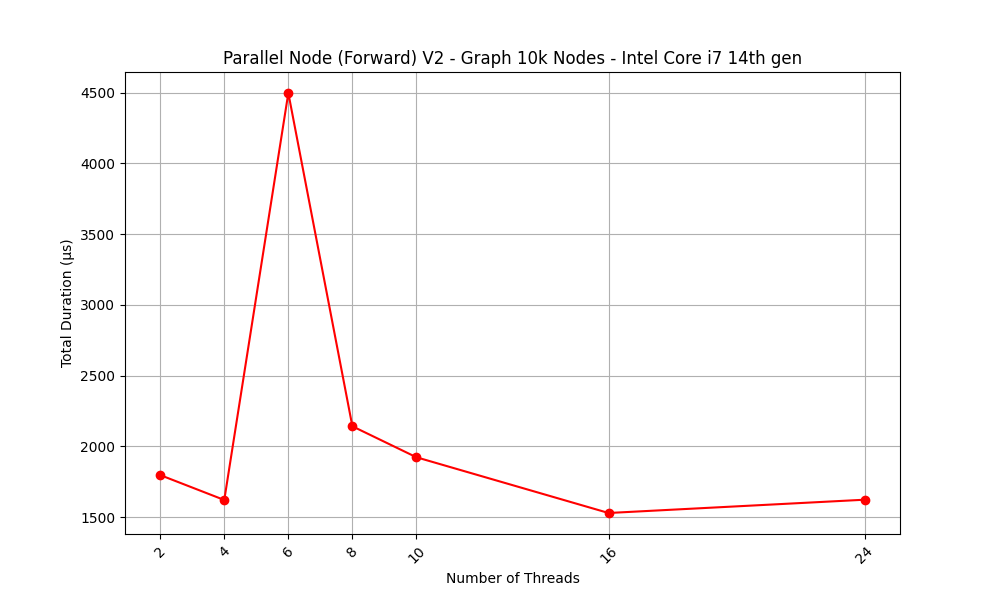
\includegraphics[width=0.52\textwidth, height=10cm, keepaspectratio]{charts/Parallel Node (Forward) V2 - Graph 10k Nodes - Intel Core i7 14th gen.png}
If we compare the two versions of the parallel algorithm, using this same graph, we can see that with every number of threads used we have a significant reduction of time, \textbf{approximately 3 orders of magnitude lower.}
In addition, using the adjacency list representation gives us the possibility to test much bigger graphs. Here are the results using graphs having 1 million of nodes:
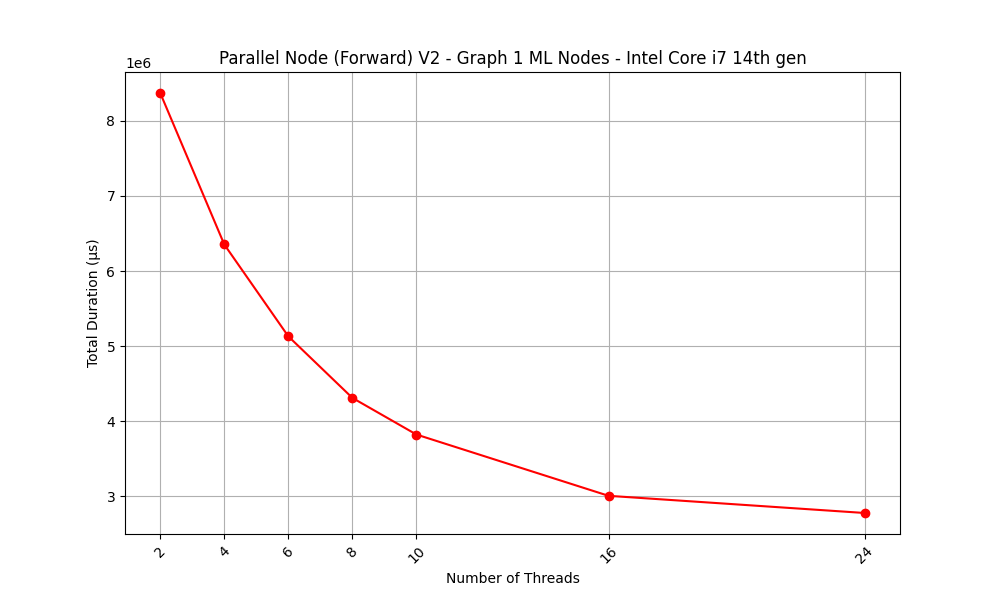
\includegraphics[width=0.52\textwidth, height=10cm, keepaspectratio]{charts/Parallel Node (Forward) V2 - Graph 1 ML Nodes - Intel Core i7 14th gen.png}


%Head 2
\section{Edge Iterator Algorithm}

The Edge Iterator Algorithm, often referred to as a variant of the Forward Algorithm for triangle counting, takes a different approach to traverse the graph compared to the node-centric iteration. It focuses directly on processing each edge in the graph to identify triangle closures.

A core principle shared with some optimized node iterator algorithms is the use of a specific vertex ordering (ranks), typically based on degree (from highest to lowest), to avoid redundant counting and optimize the search. This ordering creates a "forward" direction for edges and relationships.

In this algorithm, for each edge $(u, v)$ such that $rank(u) < rank(v)$, the algorithm seeks a third vertex $w$ that is a common neighbor of both $u$ and $v$, and also satisfies the condition $rank(w) > rank(v)$. If such a $w$ exists, then $(u, v, w)$ forms a triangle. Each triangle is counted exactly once due to this strict rank-based ordering.

To facilitate efficient and non-redundant iteration, the implementation introduces a dedicated \texttt{edgeSet}. This set stores all unique edges in the graph. In our C++ implementation, this is achieved using an \texttt{unordered\_set<Edge>} (where \texttt{Edge} is a custom struct with a specialized hash function to handle \texttt{(u,v)} and \texttt{(v,u)} as the same edge). While the \texttt{edgeSet} itself doesn't directly enforce the rank condition during its creation, the \texttt{EdgeIteratorAlgorithm} function applies the rank check (\texttt{if (ranks.at(v0) > ranks.at(v1)) \{ swap(v0, v1); \}} and \texttt{if (ranks.at(v) > ranks.at(v1))}) during its iteration to ensure that each triangle is counted exactly once according to the forward algorithm's principles. This allows a clean iteration over graph edges, decoupling the triangle counting logic from the underlying graph representation.

A crucial aspect of this algorithm's efficiency lies in how it finds common neighbors. For each edge $(u, v)$ being considered, the algorithm retrieves the \textit{full} adjacency lists (neighbors) of both $u$ and $v$. The intersection of these two adjacency lists (\texttt{neighborsV0} and \texttt{neighborsV1}) yields the set of common neighbors. Each node $w$ in this intersection forms a triangle with $u$ and $v$, provided the rank condition ($rank(w) > rank(v)$) is met.

Compared to the basic Node Iterator version, the Edge Iterator offers several advantages:

\begin{itemize}
    \item \textbf{Fewer iterations:} Instead of looping over all nodes and then all pairs of their neighbors, the algorithm directly processes each edge. This can significantly reduce the total number of primary iterations, especially in sparse graphs where $M$ (number of edges) is much smaller than $N^2$.
    \item \textbf{Direct Edge Processing:} The algorithm's focus on edges makes it naturally suited for sparse graphs, where the work done is proportional to the number of existing connections rather than potential connections.
    \item \textbf{Efficiency with Ordered Neighbors:} When adjacency lists are used and sorted (either explicitly or implicitly through data structures like \texttt{std::set} or by sorting \texttt{std::vector} neighbors), finding the intersection of neighbor lists can be very efficient, often linear in the size of the smaller list.
\end{itemize}

As with the Node Iterator, we implemented two versions of the Edge Iterator Algorithm, primarily differing in their underlying graph representation:

\begin{itemize}
    \item In \texttt{seq\_edge\_it\_v1.cpp}, the graph is stored as an adjacency matrix (\texttt{std::vector<std::vector<int>>}). Neighbor retrieval involves scanning a row of the matrix, which can be inefficient for sparse graphs. The space complexity is $\mathcal{O}(N^2)$.
    \item In \texttt{seq\_edge\_it\_v2.cpp}, an adjacency list is used, implemented as \texttt{std::map<int, std::vector<int>>}. This representation is generally more efficient for sparse graphs. Retrieving neighbors from a \texttt{std::map} takes $\mathcal{O}(\log N)$ for the map lookup plus $\mathcal{O}(d(u))$ to access the vector of neighbors. The intersection between neighbor lists (which are \texttt{std::vector<int>} here) is performed using \texttt{std::set\_intersection} after sorting, or by direct two-pointer intersection if the vectors are kept sorted.
\end{itemize}

Overall, the Edge Iterator Algorithm, especially when combined with an adjacency list representation and degree-based ordering, often provides a more efficient approach to triangle counting in terms of both time and space complexity, particularly for large and sparse graph datasets.

\begin{table}[htbp]
    \centering
    \caption{Summary of Sequential Edge Iterator Algorithm Implementation Complexities}
    \label{tab:edge_complexity_summary}
    \begin{tabular}{|l|l|}
        \hline
        \textbf{Graph Representation} & \textbf{Overall Time Complexity} \\
        \hline
        Adjacency Matrix & $\mathcal{O}(N^3)$ \\
        Adjacency List & $\mathcal{O}(M \cdot d_{\text{max}})$ \\
        \hline
    \end{tabular}
    \vspace{0.5em}
    \small
    Where $N$ is the number of vertices, $M$ is the number of edges, and $d_{\text{max}}$ is the maximum degree in the graph.
\end{table}


%Head 3
\section{Parallel Edge Iterator Algorithm}

To leverage modern multi-core processor architectures and further improve performance, the Edge Iterator Algorithm was parallelized using C++ threads. The inherent independence of processing individual edges makes this algorithm particularly well-suited for parallelization. Each triangle $(u, v, w)$ is uniquely identified by the ordered triplet of its vertices (e.g., based on ranks), ensuring that no two edges can lead to the discovery of the same triangle in an overlapping manner that would require complex synchronization for counting.

The parallelization strategy involves distributing the workload among multiple threads. Instead of a single thread iterating through the entire \texttt{edgeSet}, the set of all edges is divided into contiguous chunks. Each thread is then assigned a specific range of edges to process. This task-parallel approach allows multiple edges to be evaluated concurrently, significantly accelerating the triangle counting process.

The core logic within the \texttt{EdgeIteratorAlgorithm} function remains largely similar to its sequential counterpart. Each thread continues to perform the following steps for its assigned subset of edges:
\begin{itemize}
    \item Retrieve an edge $(u, v)$ from its assigned chunk.
    \item Apply the rank-based ordering to ensure $rank(u) < rank(v)$.
    \item Obtain the adjacency lists of $u$ and $v$.
    \item Compute the intersection of these two adjacency lists to find common neighbors.
    \item For each common neighbor $w$ that satisfies $rank(w) > rank(v)$, increment the global triangle count.
\end{itemize}
The primary modification for parallel execution lies in the handling of the global triangle count. Since multiple threads concurrently update this shared variable, an atomic counter (\texttt{std::atomic<int> countTriangles}) is employed. This guarantees thread-safe increments without the need for explicit locks, minimizing overhead and avoiding race conditions, thus preserving the correctness of the final triangle count.

The benefits of this parallel approach are substantial:
\begin{itemize}
    \item \textbf{Improved Performance:} By dividing the total work among multiple processor cores, the execution time for large graphs can be drastically reduced, leading to higher throughput.
    \item \textbf{Scalability:} The algorithm can scale effectively with the number of available CPU cores, allowing for faster processing on systems with more parallel resources.
    \item \textbf{Efficient Resource Utilization:} Parallel execution makes better use of modern hardware, which often features numerous cores.
\end{itemize}
As observed in the sequential versions, the choice of graph representation continues to influence performance. \texttt{parallel\_edge\_it\_v1.cpp} utilizes an adjacency matrix, which, despite parallelization, still incurs overhead due to linear scans for neighbor retrieval on sparse graphs. \texttt{parallel\_edge\_it\_v2.cpp}, employing adjacency lists (\texttt{std::map<int, std::vector<int>>}), is generally more efficient for sparse graphs, as neighbor lookups and intersections benefit from the optimized data structure even in a parallel context. The parallelization primarily reduces the total wall-clock time by concurrently performing these per-edge operations.


%Head 4
\section{CUDA Parallel Edge Iterator Algorithm}

The inherent massive parallelism of graph algorithms, particularly those involving independent computations per edge, makes them exceptionally well-suited for execution on Graphics Processing Units (GPUs) using NVIDIA's CUDA platform. GPUs, with their thousands of arithmetic logic units (ALUs) and high memory bandwidth, can process a multitude of edges concurrently, offering a significant performance advantage over multi-threaded CPU implementations, especially for very large graphs.

In our CUDA implementations of the Edge Iterator Algorithm, the fundamental principle of iterating through edges and identifying common neighbors based on ranked ordering remains consistent. However, the execution model shifts from CPU threads to CUDA kernels, where thousands of GPU threads (organized into blocks and grids) perform the operations. Each GPU thread is typically assigned to process one or more edges. The common global triangle count is managed via atomic operations (\texttt{atomicAdd}) to ensure correctness across concurrent thread increments. The graph's adjacency information is transferred to device memory, often in a Compressed Sparse Row (CSR) format, for efficient access by the GPU kernels.

We explored several distinct CUDA versions, primarily differing in their strategy for finding common neighbors and their utilization of GPU memory hierarchies:

\begin{itemize}
    \item \texttt{cuda\_edge\_it\_v1}: This initial version implements the intersection of neighbor lists using nested loops within each GPU thread. While simple, this approach can be inefficient for longer neighbor lists, as it involves a quadratic complexity for the intersection operation itself. All data access for neighbor lists occurs directly from global device memory.
    \item \texttt{cuda\_edge\_it\_v1\_1}: This version extends \texttt{v1} by introducing multiple kernel launches. Instead of launching one large kernel for all edges, the edges are chunked, and the kernel is launched multiple times, processing one chunk per launch. This can sometimes improve GPU occupancy and resource management, especially for graphs with highly varying node degrees, but the core intersection logic remains the same as \texttt{v1}.
    \item \texttt{cuda\_edge\_it\_v1\_2}: This variant explicitly leverages shared memory for neighbor list intersection. For each edge, threads within a block cooperatively load the neighbor lists of the edge's endpoints into dynamically allocated shared memory. After a synchronization barrier (\texttt{\_\_syncthreads()}), a single thread (e.g., \texttt{threadIdx.x == 0}) then performs the nested-loop intersection on this much faster shared data. A fallback mechanism ensures that if the combined size of the neighbor lists exceeds the available shared memory, the intersection is performed directly from global memory. This aims to reduce global memory latency for smaller neighbor lists.
    \item \texttt{cuda\_edge\_it\_v2}: This is a more optimized version that, after ensuring neighbor lists are sorted (a preprocessing step on the host), employs a two-pointer merge-like algorithm for finding the intersection of neighbor lists within each GPU thread. This approach has a linear time complexity proportional to the sum of the degrees of the two vertices, making it significantly more efficient than nested loops for intersection, even when accessing global memory.
    \item \texttt{cuda\_edge\_it\_v2\_1}: Building upon \texttt{v2}, this version explicitly incorporates shared memory for the merge-like intersection. Each block processes a single edge, and threads within that block cooperatively load the neighbor lists into shared memory before a single thread performs the merge-intersection. This aims to reduce global memory latency, benefiting edges whose neighbor lists fit into shared memory.
    \item \texttt{cuda\_edge\_it\_v2\_2}: This version also utilizes shared memory with the merge-like approach, but with a different thread-to-edge mapping. Multiple edges can be processed within a single thread block, and each thread processes its own edge, dynamically allocating shared memory space for its neighbor lists. This can be more flexible for varying list sizes across different threads within the same block.
\end{itemize}

The key advantage of CUDA lies in its ability to exploit fine-grained data parallelism. When a single edge calculation (intersection of two neighbor lists) is independent of other edge calculations, thousands of these operations can proceed in parallel, leading to dramatic speedups compared to CPU-based parallel implementations. This is especially true when neighbor lists are short to moderate and fit well into GPU memory hierarchies (as in \texttt{v1\_2}, \texttt{v2\_1}, \texttt{v2\_2}), or when optimized intersection algorithms like the two-pointer approach (\texttt{v2}, \texttt{v2\_1}, \texttt{v2\_2}) are employed. The efficiency gains are particularly pronounced for dense graphs or graphs with many edges where the cost of data transfer to the GPU is amortized over a large amount of parallel computation.






\section{SUMMARY}
summary todo \cite{DEK3}, \cite{DEK4}.

\section{CONCLUSION}
conclusion todo~\cite{DEK5}.

\section{ACKNOWLEDGMENT}
acknowledgment todo

\bibliography{aes2e.bib}
\bibliographystyle{aes2e.bst}

% NOTE:
% - in case you are not using bibTex you have to manually edit the bibliograpy as below.
% - if submitting a bibTex file is not allowed you can copy the content from the aes2e.bbl file  
%\begin{thebibliography}{99}
%
%\newcommand{\enquote}[1]{``#1''}
%\providecommand{\url}[1]{\texttt{#1}}
%\providecommand{\urlprefix}{URL }
%\expandafter\ifx\csname urlstyle\endcsname\relax
%  \providecommand{\doi}[1]{[Online]. Available: \discretionary{}{}{}#1}\else
%  \providecommand{\doi}{doi:\discretionary{}{}{}\begingroup
%  \urlstyle{rm}\Url}\fi
%
%\bibitem{DEK1}
%D.~Preis, \enquote{Phase Distortion and Phase Equalization in Audio Signal
%  Processing---A Tutorial Review,} \emph{J. Audio Eng. Soc.}, vol.~30, no.~11,
%  pp. 774--779 (1982 Nov.).
%
%\bibitem{DEK2}
%J.~S. Abel, D.~P. Berners, \enquote{MUS424/EE367D: Signal Processing Techniques
%  for Digital Audio Effects,}  (2005), unpublished Course Notes, CCRMA,
%  Stanford University, Stanford, CA.
%
%\bibitem{DEK3}
%C.~Roads, \enquote{Musical Sound Transformation by Convolution,} presented at
%  the \emph{Int. Computer Music Conf.}, pp. 102--109 (1993).
%
%\bibitem{DEK4}
%C.~Roads, \emph{The Computer Music Tutorial} (MIT Press, Cambridge, MA), 1st
%  ed. (1996).
%
%\bibitem{DEK5}
%H.~Morgenstern, B.~Rafaely, \enquote{Spatial Reverberation and Dereverberation
%  Using an Acoustic Multiple-Input Multiple-Output System,} \emph{J. Audio Eng.
%  Soc}, vol.~65, no. 1/2, pp. 42--55 (2017 Jan.Feb.),
%  \doi{https://doi.org/10.17743/jaes.2016.0063}.
%  
%\end{thebibliography}

%Appendix
\appendix
\section*{APPENDIX}
appendix todo


\begin{nomenclature}[PAMPs]
\subsection*{NOMENCLATURE}
\nomentry{a$_c$}{condensation coefficient condensation coefficient condensation coefficient}


\nomentry{TLR}{Toll-like receptor}

\nomentry{PAMPs}{pathogen-associated molecular patterns condensation coefficient condensation}
\end{nomenclature}

%Biography
 \biography{A1firstname A1lastname}{a.eps}{A1firstname A1lastname is professor of audio signal processing at Helsinki University of Technology (TKK), Espoo, Finland. He received his Master of Science in Technology, Licentiate of Science in Technology, and Doctor of Science in Technology degrees in electrical engineering from TKK in 1992, 1994, and 1995, respectively. His doctoral dissertation dealt with fractional delay filters and physical modeling of musical wind instruments. Since 1990, he has worked mostly at TKK with the exception of a few periods. In 1996 he spent six months as a postdoctoral research fellow at the University of Westminster, London, UK. In 2001-2002 he was professor of signal processing at the Pori School of Technology and Economics, Tampere University of Technology, Pori, Finland. During the academic year 2008-2009 he has been on sabbatical and has spent several months as a visiting scholar at the Center for Computer Research in Music and Acoustics (CCRMA), Stanford University, Stanford, CA. His research interests include musical signal processing, digital filter design, and acoustics of musical instruments. Prof. V\"alim\"aki is a senior member of the IEEE Signal Processing Society and is a member of the AES, the Acoustical Society of Finland, and the Finnish Musicological Society. He was the chairman of the 11th International Conference on Digital Audio Effects (DAFx-08), which was held in Espoo, Finland, in 2008.}
 \biography{A2firstname A2lastname}{b.eps}{A2firstname A2lastname is a consulting professor at the Center for Computer Research in Music and Acoustics (CCRMA) in the Music Department at Stanford University where his research interests include audio and music applications of signal and array processing, parameter estimation, and acoustics. From 1999 to 2007, Abel was a co-founder and chief technology officer of the Grammy Award-winning Universal Audio, Inc. He was a researcher at NASA/Ames Research Center, exploring topics in room acoustics and spatial hearing on a grant through the San Jose State University Foundation. Abel was also chief scientist of Crystal River Engineering, Inc., where he developed their positional audio technology, and a lecturer in the Department of Electrical Engineering at Yale University. As an industry consultant, Abel has worked with Apple, FDNY, LSI Logic, NRL, SAIC and Sennheiser, on projects in professional audio, GPS, medical imaging, passive sonar and fire department resource allocation. He holds Ph.D. and M.S. degrees from Stanford University, and an S.B. from MIT, all in electrical engineering. Abel is a Fellow of the Audio Engineering Society.}
\end{document}